\documentclass[tikz]{standalone}
\usepackage{amsmath}
\definecolor{bgcol}{HTML}{171D2B}
\definecolor{accent}{HTML}{F7B538}
\definecolor{setcol}{HTML}{7DA2C9}
\pagecolor{bgcol}
\begin{document}
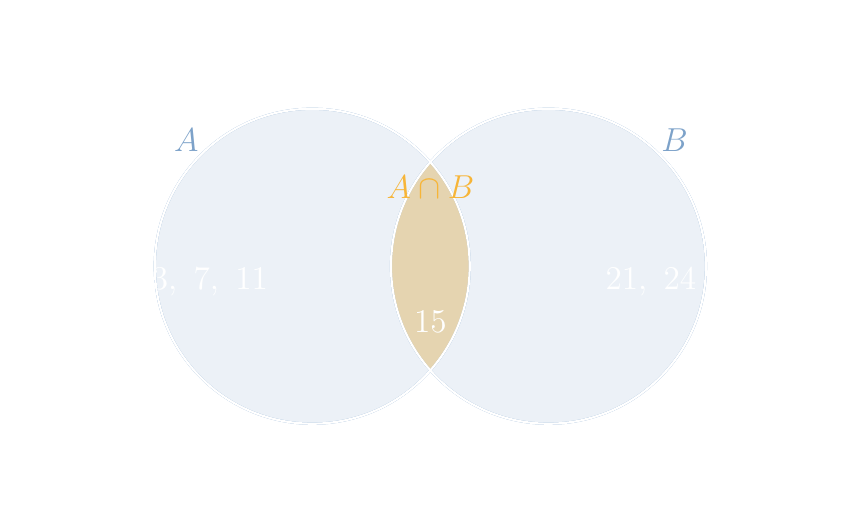
\begin{tikzpicture}[scale=1.0, color=white, font=\large]
  % Diagram Venn: A irisan B, dua lingkaran dengan jelas
  \draw[thick, setcol, fill=setcol, fill opacity=0.15] (0,0) circle (2);
  \draw[thick, setcol, fill=setcol, fill opacity=0.15] (3,0) circle (2);
  % irisan disorot
  \begin{scope}
    \clip (0,0) circle (2);
    \fill[accent, fill opacity=0.35] (3,0) circle (2);
  \end{scope}
  \draw[thick] (0,0) circle (2);
  \draw[thick] (3,0) circle (2);
  \draw[thick] (-3.6,-3) rectangle (6.6,3);
  \node[anchor=south west] at (-3.4,2.5) {$S$};
  \node[setcol] at (-1.6,1.6) {$A$};
  \node[setcol] at (4.6,1.6) {$B$};
  \node[accent] at (1.5,1.0) {$A \cap B$};
  \node at (-1.3,-0.2) {$3,\ 7,\ 11$};
  \node at (1.5,-0.7) {$15$};
  \node at (4.3,-0.2) {$21,\ 24$};
\end{tikzpicture}
\end{document}